\documentclass{beamer}
\usetheme{Madrid}
\setbeamertemplate{bibliography item}{\insertbiblabel}

\usepackage[main=english,czech]{babel}
%\usepackage[T1]{fontenc}
\usepackage[utf8]{inputenc}
\usepackage{url}
\usepackage{caption}
\usepackage{graphicx}
\usepackage{xcolor}

\captionsetup[figure]{font=footnotesize, justification=justified, format=hang}

%\usepackage{biblatex}
%\addbibresource{references.bib}

\AtBeginSection[]
{
	\begin{frame}<beamer>[noframenumbering]
		\frametitle{Outline}
		\tableofcontents[currentsection]
	\end{frame}
}

\title[OFTPC track simulation \& reconstruction]{Simulation and reconstruction of charged particle trajectories in an orthogonal fields time projection chamber (OFTPC)}
%\subtitle{Subtitle}
\author[M.~Vavřík]{\foreignlanguage{czech}{Martin Vavřík}\vspace{0.5cm}\\martin.vavrik@cvut.cz\\IEAP CTU PRAGUE\\}
\logo{
\includegraphics[width=0.08\textwidth]{../images/logo}}
\date{4\textsuperscript{th} - 8\textsuperscript{th} December, 2023}

\begin{document}
	
	\begin{frame}
		\titlepage
	\end{frame}
	
	\begin{frame}
		\frametitle{Outline}
		\tableofcontents
	\end{frame}
	
	\section{Motivation}
	\begin{frame}
		\frametitle{Motivation}
		\begin{itemize}
			\item Measurement of anomalies in angular correlation of electron and positron internally produced in excited $ {}^8\text{Be} $ and $ {}^4\text{He} $
				\begin{columns}
				\column{0.45 \textwidth}
				\begin{figure}
					\centering
					\begin{minipage}[t][4.3cm]{\textwidth}
						\centering
						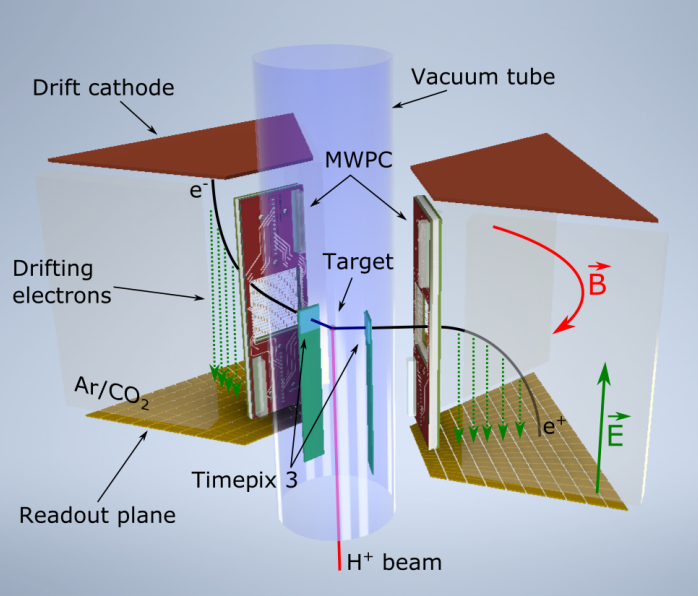
\includegraphics[width=0.81\linewidth]{../images/diagram.png}\newline
					\end{minipage}
					\caption{Two out of the six TPC chambers.\cite{poster}}
					\label{fig:dia}
				\end{figure}
				\column{0.45 \textwidth}
				\begin{figure}
					\centering
					%$ $\newline
					\begin{minipage}[t][4.3cm]{\textwidth}
						\centering
						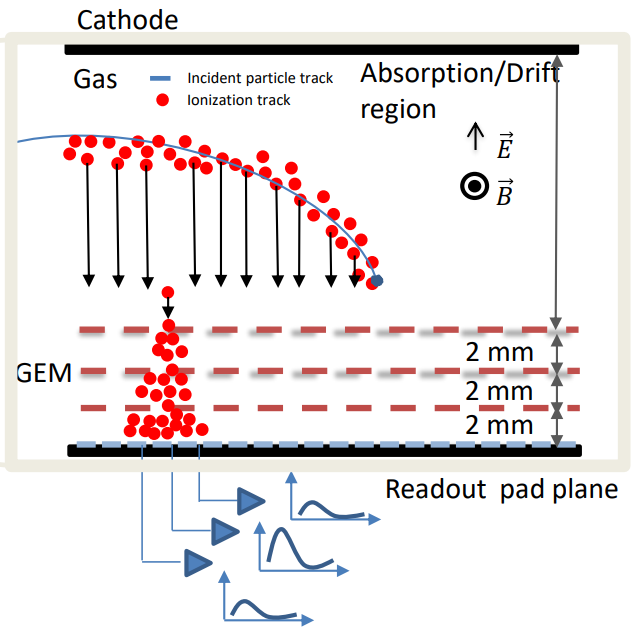
\includegraphics[width=0.81\linewidth]{../images/diagram2.png}\newline
					\end{minipage}
					\caption{TPC with triple gas electron multiplier (GEM) readout.\cite{poster}}
					\label{fig:dia2}
				\end{figure}
				\end{columns}
		\end{itemize}
	\end{frame}

	\begin{frame}
		\frametitle{X17 detector}
		\begin{itemize}
			\item For energy reconstruction, tracks in the time projection chamber (TPC) will be used
			\begin{itemize}
				\item Atypical TPC (magnetic field is perpendicular instead of parallel to electric)
				\item This interferes with the direction of the drift of electrons
				\item Energy can be determined using curvature of the track in the inhomogeneous magnetic field
				\item Magnetic field data from simulation is used
			\end{itemize}
			\item \textcolor{red}{Less information about how TPCs work, more information about reasons for OFTPC.}
		\end{itemize}
	\end{frame}
	
	\section{Track simulation}
	\begin{frame}
		\frametitle{Track simulation}
		\begin{itemize}
			\item We use Garfield++ for track simulation
			\begin{itemize}
				\item Primary relativistic particle simulated using Heed program~\cite{heed}
				\item Secondary ionization electrons simulated using microscopic tracking (uses equation of motion)
				\begin{itemize}\item Relatively slow (typically 5-30 CPU hours per track), very precise especially for small structures.  \end{itemize}
			\end{itemize}
			\item Batches of 9702 tracks with different initial parameters simulated on MetaCentrum
			\begin{itemize}
				\item Electron or positron
				\item 11 different energies (from 3~MeV to 11~MeV)
				\item 21 different angles~$\varphi$ and 21 different angles~$\theta$ (see picture on next slide)
			\end{itemize}
		\end{itemize}
	\end{frame}
	
	\begin{frame}
		\frametitle{Track simulation}
		\begin{figure}
			\centering
			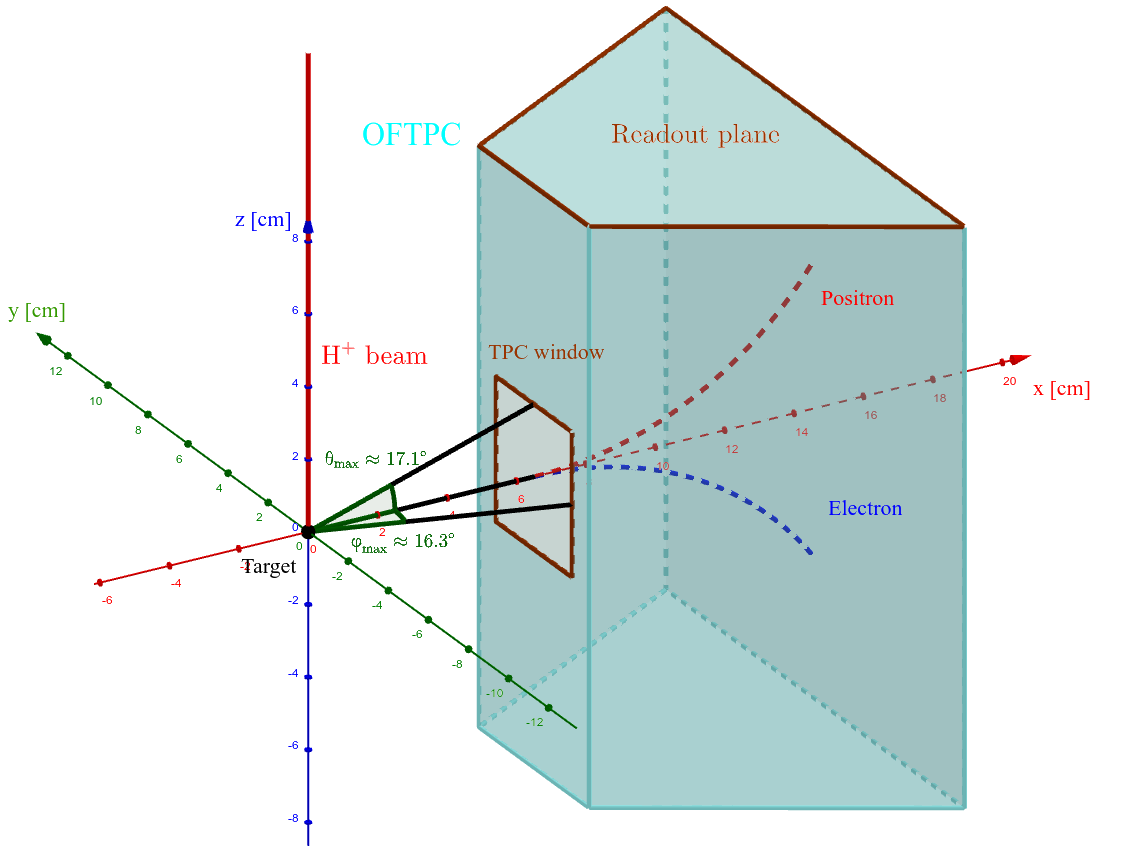
\includegraphics[width = 0.9 \linewidth]{../images/tpc_micro_simulation.png}
			\caption{Diagram of the batch simulation parameters, $\theta \in [-17.1^\circ,17.1^\circ]$, $\varphi \in [-16.3^\circ,16.3^\circ]$, $ E_k \in [3,13] $~MeV.}
		\end{figure}
	\end{frame}
	
	\begin{frame}
		\frametitle{Simulated track example (microscopic tracking)}		
		\begin{columns}
			\column{0.33\textwidth}
			\begin{figure}
				\centering
				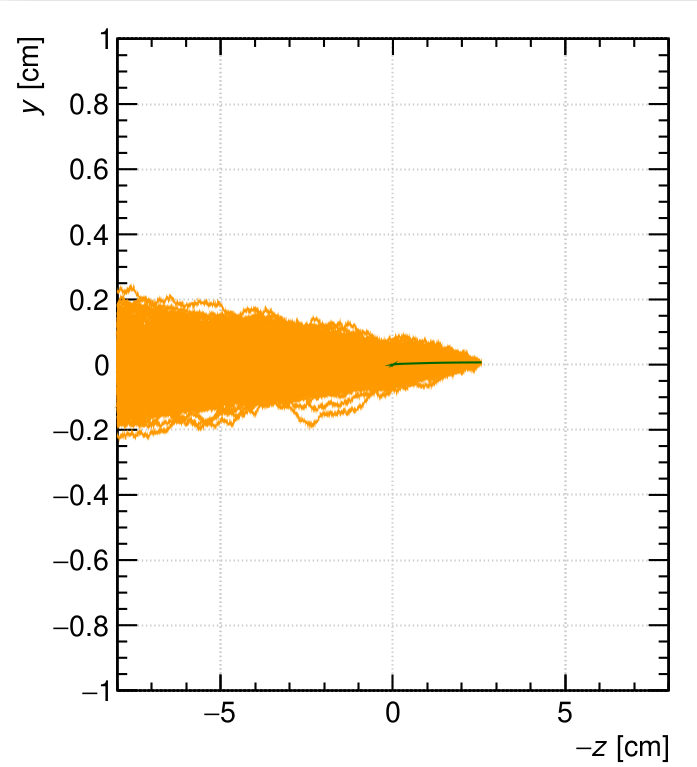
\includegraphics[width = 0.95 \linewidth]{../images/track1.png}
				\caption{Diffusion front view}
			\end{figure}
			\column{0.33\textwidth}
			\begin{figure}
				\centering
				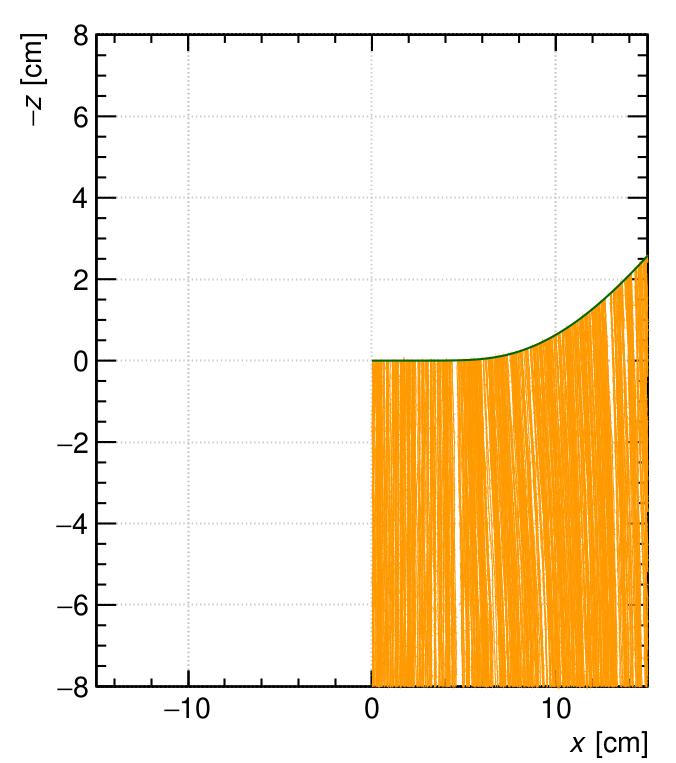
\includegraphics[width = 0.95 \linewidth]{../images/track2.png}
				\caption{Electron drift}
			\end{figure}
			\column{0.33\textwidth}
			\begin{figure}
				\centering
				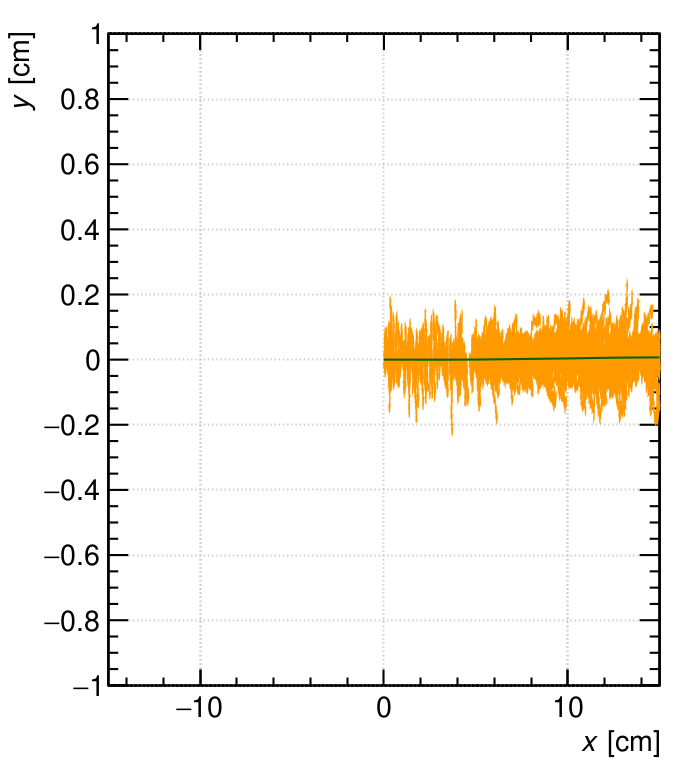
\includegraphics[width = 0.95 \linewidth]{../images/track3.png}
				\caption{Diffusion top view}
			\end{figure}
		\end{columns}
	\end{frame}

	\begin{frame}
		\frametitle{Ionization electrons map simulation}
		\begin{itemize}
			\item In the experimental setup TPC only detects secondary ionization electrons (after multiplication on triple GEM)
			\item These electrons drift at a~constant velocity towards the readout plane
			\item We can use a~simulation of evenly spaced electrons for the reconstruction (time consuming -- run on MetaCentrum)
			\begin{itemize}
				\item Current spacing 5~mm, 100 electrons simulated in each location with 0.1~eV energy in a~random direction
			\end{itemize}
		\end{itemize}
		\begin{figure}
			\centering
			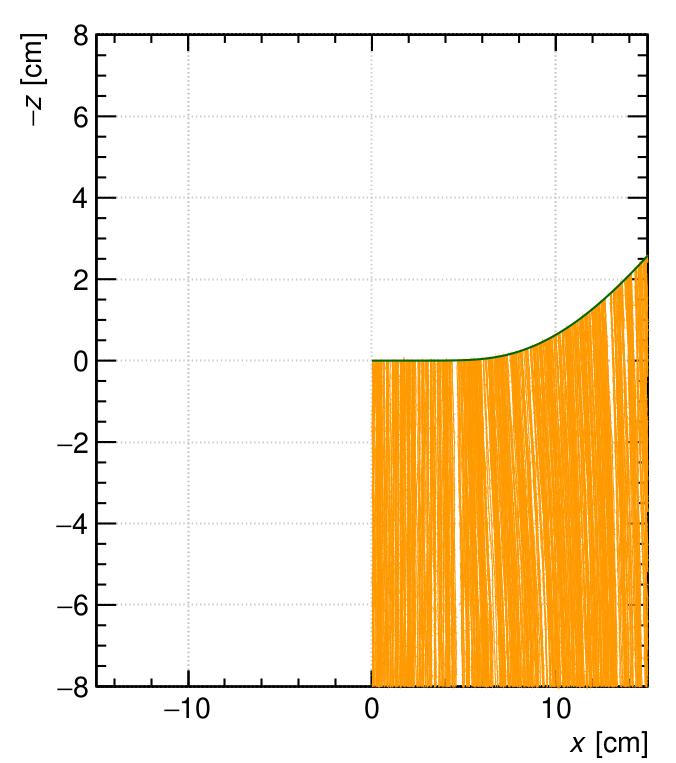
\includegraphics[width = 0.3 \linewidth]{../images/track2.png}
			\caption{Electron drift}
		\end{figure}
	\end{frame}

	\begin{frame}
		\frametitle{Ionization electron map simulation}
		\begin{itemize}
			\item As a result we get an approximation of a mapping from initial coordinates of the electrons $(x,y,z)$ to the readout coordinates $(x',y',t)$
			\item By interpolating we can get the inverse map
			\item We can use the inverse map to finally create mapping from our discrete readout values (channel number, time) to voxels of the primary track
		\end{itemize}
		\begin{figure}
			\centering
			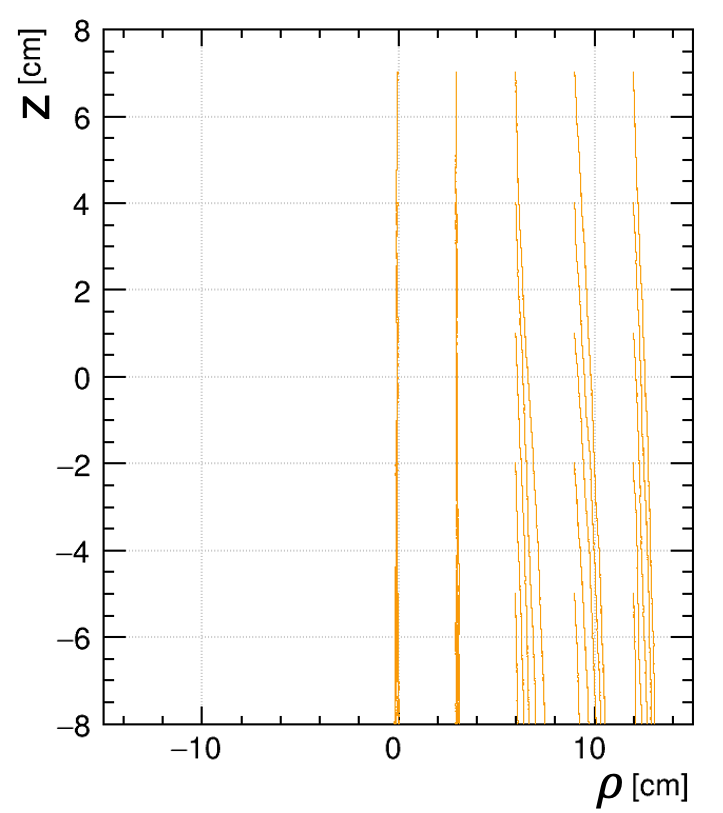
\includegraphics[height=0.4\textheight]{../images/map_lines.png}
			\caption{Partial simulation of the map}
		\end{figure}
	\end{frame}
	\begin{frame}
		\frametitle{Ionization electron map simulation}
		\begin{figure}
			\centering
			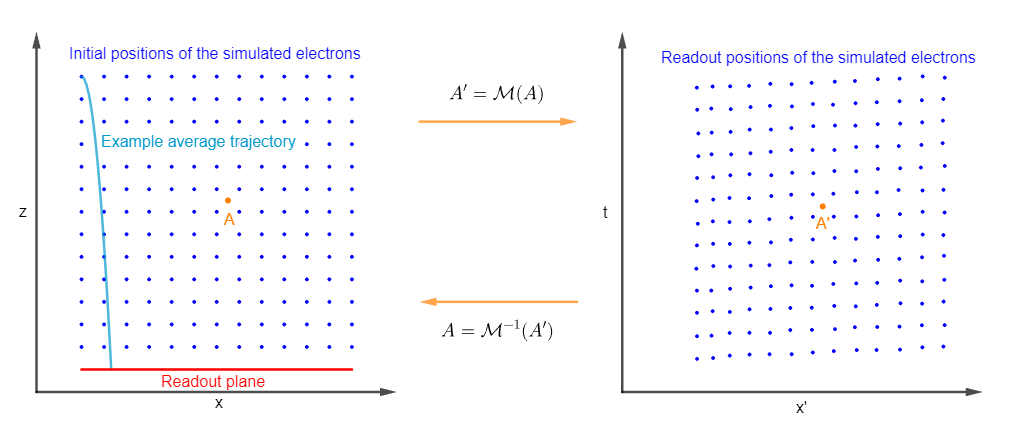
\includegraphics[width=\textwidth]{../images/map_visualization.png}
			\caption{2D visualization of the simulated mapping $\mathcal{M}$ and inverse mapping $\mathcal{M}^{-1}$.}
		\end{figure}
	\end{frame}
	\begin{frame}
		\frametitle{Ionization electron map simulation}
		\begin{figure}
			\centering
			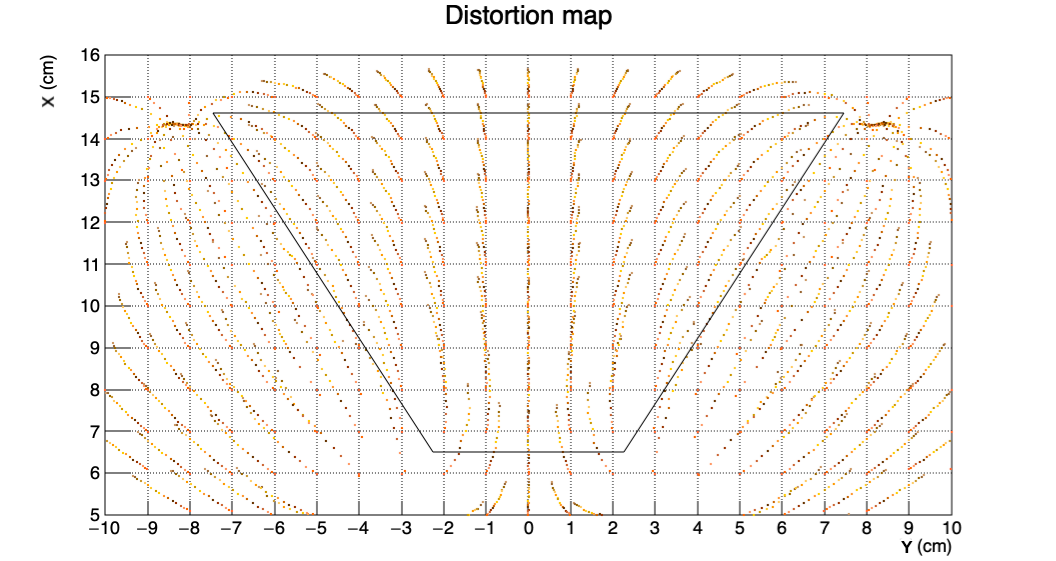
\includegraphics[height=0.6\textheight]{../images/map_dist.png}
			\caption{$x$ and $y$ coordinate distortion at different $z$ values (Credit: Hugo Natal da Luz).}
		\end{figure}
	\end{frame}
	\begin{frame}
		\frametitle{Ionization electron map simulation}
		\begin{figure}
			\centering
			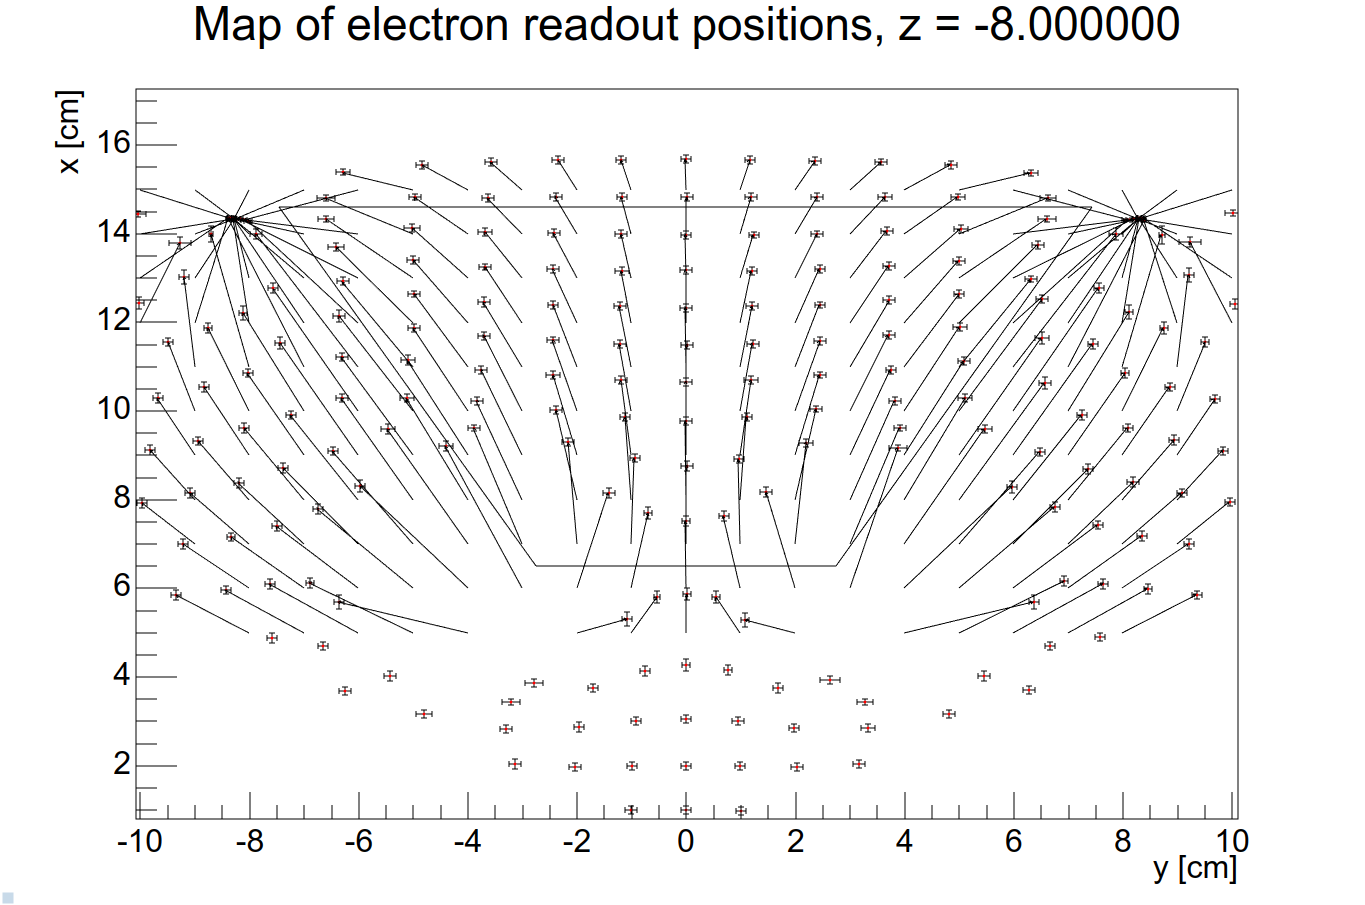
\includegraphics[height=0.65\textheight]{../images/map_dist2.png}
			\caption{$x$ and $y$ coordinate distortion for maximal initial distance from readout}
		\end{figure}
	\end{frame}
	\begin{frame}
		\frametitle{Ionization electron map simulation}
		\begin{figure}
			\centering
			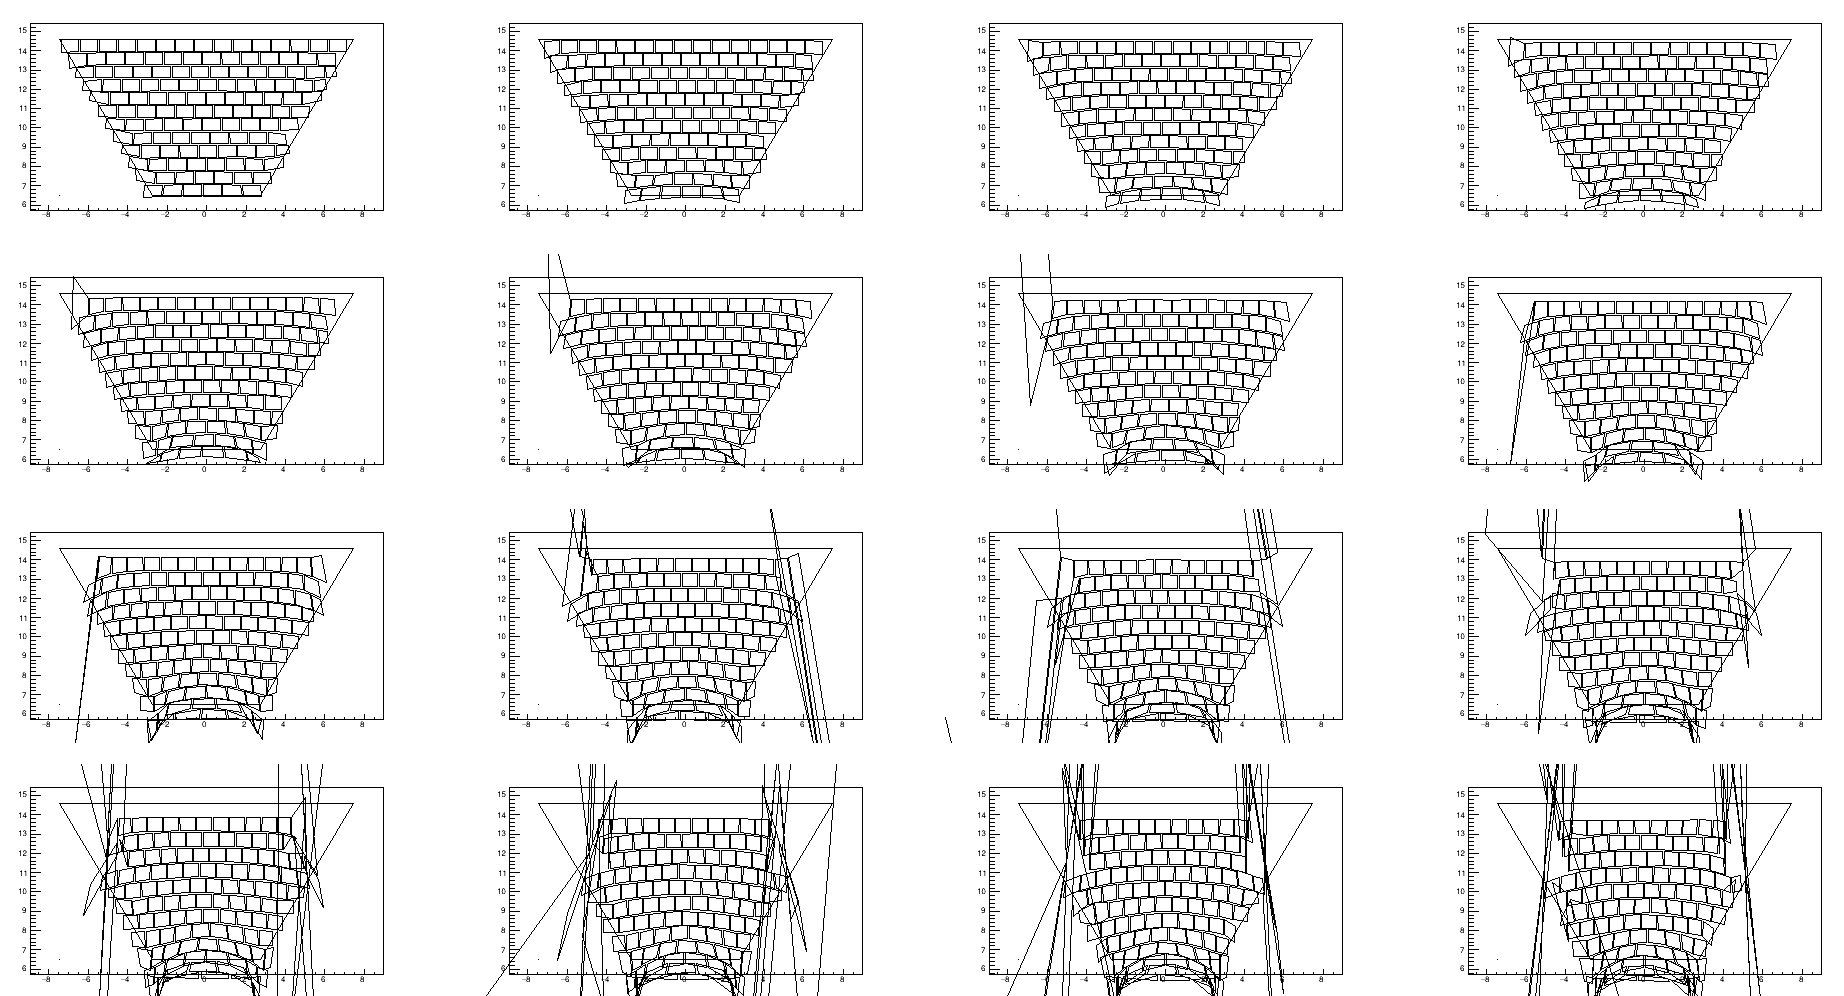
\includegraphics[height=0.68\textheight]{../images/pads_dist.png}
			\caption{Pad voxel boundaries for different times (picture of first attempt).}
		\end{figure}
	\end{frame}


	\section{Track reconstruction}
	\begin{frame}
		\frametitle{Track reconstruction}
		\begin{itemize}
			\item First attempts using only the inverse map (not accounting for readout pads)
			\item Simple reconstruction with pads and time bins, counting the number of electrons in each bin
		\end{itemize}
		\begin{figure}
			\centering
			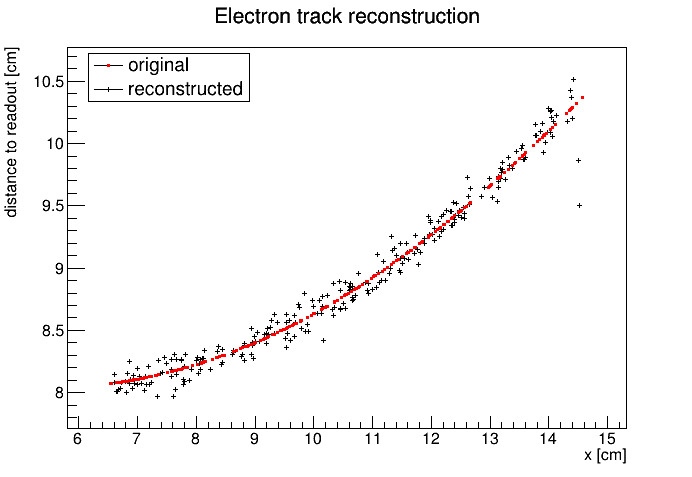
\includegraphics[width=0.6\textwidth]{../images/reco_track.png}
			\caption{Original and reconstructed interaction points on the simulated track}
		\end{figure}
	\end{frame}

	\section{Energy reconstruction}
	\begin{frame}
		\frametitle{Energy reconstruction}
		\begin{itemize}
			\item Prefit with circle with smoothly attached lines
			\item One parameter (kinetic energy) fit with 4\textsuperscript{th} order Runge-Kutta fit
			\item In both steps known initial position and direction of the particle assumed
			\item Currently cca 0.3~CPU seconds per track
		\end{itemize}
		\begin{figure}
			\centering
			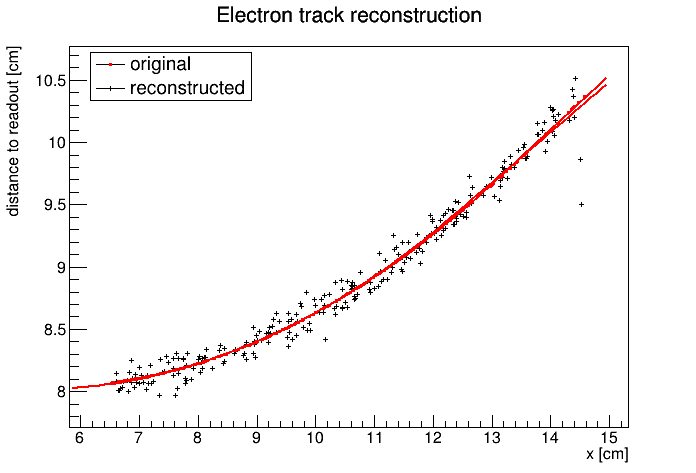
\includegraphics[width=0.5\textwidth]{../images/reco_e.png}
			\caption{8 MeV simulated electron energy reconstruction from both original and reconstructed interaction points. Results are 8.27 and 7.93 MeV.}
		\end{figure}		
	\end{frame}
	\begin{frame}
		\frametitle{Energy reconstruction precision}
		\begin{columns}
			\column{0.5\textwidth}
			\centering
			\Large \textbf{Electrons}
			\begin{figure}
				\centering
				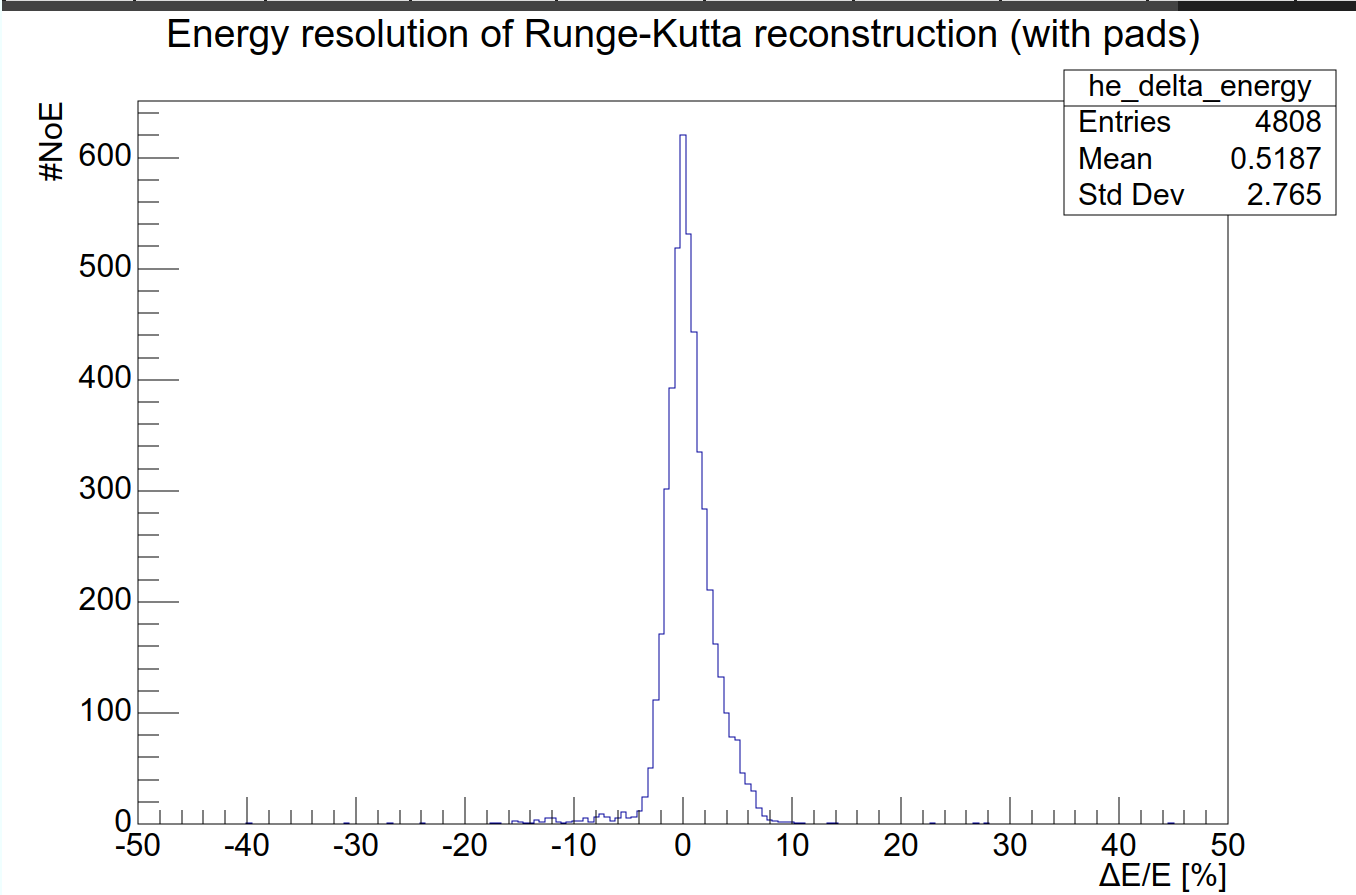
\includegraphics[width = 0.95 \linewidth]{../images/c_e_delta_energy.png}
			\end{figure}
			\column{0.5\textwidth}
			\centering
			\Large \textbf{Positrons}
			\begin{figure}
				\centering
				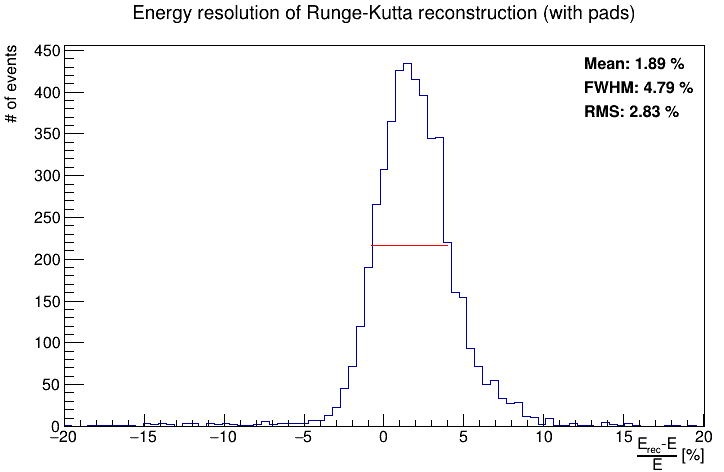
\includegraphics[width = 0.95 \linewidth]{../images/c_p_delta_energy.png}
			\end{figure}
		\end{columns}
		\captionof{figure}{Relative reconstruction deviation of the~kinetic energy of electron and positron tracks. These histograms represent the best possible resolution for our detector.}
	\end{frame}
	
	
	\section{Summary \& Future}	
	\begin{frame}
		\frametitle{Summary}
		\begin{itemize}
			\item Several batches of tracks have been simulated for testing purposes
			\item The map of secondary electron positions and drift times has been generated
			\item The map has been tested by preliminary track reconstruction
			\item Testing of the energy reconstruction has begun, first attempts of determining the resolution of our detector were made
		\end{itemize}
	\end{frame}
	\begin{frame}
		\frametitle{Future}
		\begin{itemize}
			\item Account for parasitic tracks caused by high energy secondary electrons
			\item Account for GEM in simulation, charge distribution between pads
			\item Optimize Runge-Kutta integration fit with likelihood approach (instead of least squares) if needed
			\item Write a faster simulation method for secondary electrons using the map
			\item Fix the systematic error of reconstruction discovered using the simulated tracks
		\end{itemize}
	\end{frame}
	\begin{frame}
		\frametitle{Notes (what else to mention)}
		\begin{itemize}
			\item Magnetic field simulation.
			\item Better simulated track example pictures?
			\item Extra slide with the whole process summary?
			\item Better description than pad voxels.
			\item Better description of interpolation?
			\item Residues on first attempts of track reconstruction?
			\item Change energy reconstruction figure!
			\item More energy reconstruction resolution figures.
			\item ATOMKI slide
			\item OFTPC slide (permanent magnets vs solenoid, parallel field, curving --> need higher resolution,readout electronics positioning (limited budget))
		\end{itemize}
	\end{frame}
	
	{
		%\usebackgroundtemplate{\includegraphics[width=\paperwidth,height=\paperheight]{../images/DSC_5602.jpg}}%
		\begin{frame}[noframenumbering]{}
			\begin{center}
				\Huge Thank you for your attention.
			\end{center}
		\end{frame}
	}
	
	%\section{References}
	\begin{frame}[allowframebreaks,noframenumbering]
		\frametitle{References}
		%\printbibliography
		\bibliography{../references}
		\bibliographystyle{unsrt}
	\end{frame}
	
\end{document}